\documentclass[a4paper]{article}
\usepackage[utf8]{inputenc}
\usepackage[T1]{fontenc}
\usepackage[english]{babel}
\usepackage{amsmath,amssymb,amsfonts}
\usepackage{lmodern}
\usepackage{microtype}
\usepackage{tikz}

\newcommand{\T}{\texttt{T}}
\newcommand{\F}{\texttt{F}}
\newcommand{\on}{\texttt{on}}
\newcommand{\off}{\texttt{off}}

\title{Bayesian Networks --- Exercise 1}
\author{Claudi Lleyda Moltó}

\begin{document}
\maketitle

Dr.\ Ann Nicholson spends~\(60\%\) of her work time in her office. The rest of
her work time is spent elsewhere. When Ann is in her office, half the time her
light is off (when she is trying to hide from students and get research done).
When she is not in her office, she leaves her light on only~\(5\%\) of the
time.~\(80\%\) of the time she is in her office, Ann is logged onto the
computer.  Because she sometimes logs onto the computer from home,~\(10\%\) of
the time she is not in her office, she is still logged onto the computer.

\begin{enumerate}
    \item[(a)] Construct a Bayesian network to represent the scenario just
        described.
\end{enumerate}

We start by defining appropriate random variables:
\begin{align*}
    O &= \textrm{``Dr.\ Ann Nicholson is in her office''} \\
    L &= \textrm{``The light in Dr.\ Ann Nicholson's office is on''} \\
    C &= \textrm{``Dr.\ Ann Nicholson is logged onto her computer''}
\end{align*}
where~\(O\) can be~\texttt{T} or~\texttt{F}, while~\(L\) and~\(C\) can
be~\texttt{on} or~\texttt{off}.

The variables~\(L\) and~\(C\) depend on whether Dr.\ Ann Nicholson is in her
office, while the variables~\(L\) and~\(C\) are conditionally independent. This
induces the following DAG

\begin{center}
    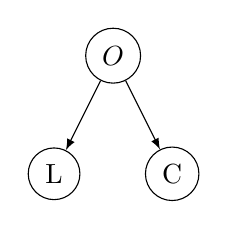
\begin{tikzpicture}[edge from parent/.style={draw,-latex}]
        \node[circle,draw](z){$O$}
            child{node[circle,draw]{L}}
            child{node[circle,draw]{C}};
    \end{tikzpicture}
\end{center}

we know the marginal distribution of~\(O\):
\begin{center}
    \begin{tabular}{cc}
        \texttt{T} & \texttt{F} \\ \hline
        \(0.6\) & \(0.4\)
    \end{tabular}
\end{center}

and the conditional distributions of~\(L\) and~\(C\) with respect to~\(O\):
\[
    \begin{array}{c|cc}
        L              & \texttt{on} & \texttt{off} \\ \hline
        O = \texttt{T} & 0.50        & 0.50 \\
        O = \texttt{F} & 0.05        & 0.95
    \end{array}
    \qquad
    \begin{array}{c|cc}
        C              & \texttt{on} & \texttt{off} \\ \hline
        O = \texttt{T} & 0.80        & 0.20 \\
        O = \texttt{F} & 0.10        & 0.90
    \end{array}
\]

We know that this DAG is a Bayesian Network because~\(L\) and~\(C\) are
conditionally independent, and we also know that the conditional distributions
and the marginal distribution of the root nodes give the joint probability
through the chain rule.

\begin{enumerate}
    \item[(b)] Suppose a student checks Dr.\ Nicholson's login status and sees
        that she is logged on. What effect does this have on the student's
        belief that Dr.\ Nicholson's light is on?
\end{enumerate}

\begin{enumerate}
    \item[(c)] Is the evidence that Dr.\ Nicholson's is logged on in favor of or
        against her light is on?
\end{enumerate}

\end{document}
